\chapter{Résultat obtenue}
\label{chap:res}

\section{Introduction}
Dans le chapitre précédent, nous avons généralement présenté des méthodes concernant notre travail avec leur implémentation détaillées. Dans ce chapitre, nous allons présenter notre résultat en comparant avec la méthode SVM standard, l'implémentation LIBSVM \cite{cl01}.

\section{Méthode SGD binaire}
Pour cette étape, nous voulons comparer SGD-SVM binaire avec LIBSVM pour voir si quelle méthode est plus efficace. Nous utilisons ci-dessous la base de données binaire (2 classes) de LIBSVM \cite{svmdata1}, Adult avec la taille d'exemple d'entrées différente.\\

Dans cette expérimentation, nous avons utilisé la fonction linaire de SVM car elle est plus efficace que les autre fonctions (seulement avec cette base de données). Pour la méthode SGD, nous avons utilisé $T = 10000$ cycles et chaque cycle nous choisissons 10 exemples. Avec cette méthode, le résultat change un peu (moins de 10\%) chaque case de test car elle choisit aléatoire des exemples dans chaque cycle, donc, nous avons testé 10 fois chaque exemple et fait la moyenne pour comparer avec la méthode SVM.

\begin{table}
\begin{center}
    \begin{tabular}{ | c | c | c | c | c | c | c |}
    \hline
    Données & \#Exemple & LIBSVM(\%) & SGD(\%) & LIBSVM(s) & SGD(s) & $\frac{SVM(s)}{SGD(s)}$ \\ \hline
    
    a1a & 1,605 & 83.82 & 84.30 & 0.438 & 0.044 & 10 \\ \hline
    
    a2a & 2,265 & 84.27 & 84.48 & 0.826 & 0.045 & 18 \\ \hline
    
    a3a & 3,185 & 84.33 & 84.31 & 6.990 & 0.050 & 139 \\ \hline
    
    a4a & 4,781 & 84.44 & 84.33 & 3.162 & 0.043 & 73 \\ \hline
    
    a5a & 6,414 & 84.39 & 84.33 & 5.766 & 0.048 & 120 \\ \hline
    
    a6a & 11,220 & 84.72 & 84.34 & 20.846 & 0.049 & 425 \\ \hline
    
    a7a & 16,100 & 84.83 & 84.45 & 42.392 & 0.056 & 757 \\ \hline
    
    a8a & 22,696 & 85.16 & 84.95 & 91.500 & 0.054 & 1,694 \\ \hline
    
    a9a & 32,561 & 84.97 & 84.64 & 299.648 & 0.064 & 4,682 \\ \hline
    
    \end{tabular}
\end{center}
\caption{Comparaison entre LIBSVM et SGD-SVM}
\label{tab:svmsgd}
\end{table}

\begin{figure}[ht!]
\centering
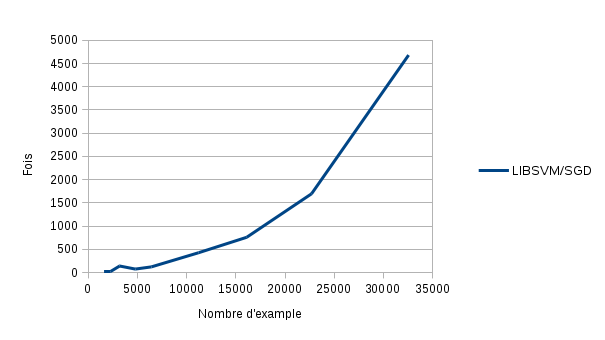
\includegraphics[width=150mm]{images/res}
\caption{Comparaison de la vitesse entre LIBSVM et SGD binaire}
\label{fig:res}
\end{figure}

\pagebreak
Par rapport au table \ref{tab:svmsgd}, nous trouvons que le taux de classification de SGD-SVM et SVM est presque pareil tandis que le temps d'apprendre est différent. La vitesse de SGD-SVM est très vite que la vitesse de SVM standard. Cet avantage de SGD-SVM est plus claire quand le nombre d'exemples d'apprentissage augmente. Cette chiffre est démontrée dans la colonne de table \ref{tab:svmsgd} ou aussi dans le figure \ref{fig:res}.\\

Les données que nous avons utilisé ont 123 caractéristiques. Nous trouvons que quand le nombre d'exemple est de 1,605, la méthode SGD est plus vitesse que la méthode SVM 10 fois, mais quand le nombre d'exemple de 32,561, SGD plus vitesse que SVM 4,682 fois. Ce chiffre confirme que la méthode SGD est beaucoup plus vitesse que SVM, surtout pour les grandes données. Donc, la méthode SGD s'adapte mieux au problème de classification d'image dont la base de données est très grande. En raison de son avantage, nous voulons la développer pour qu'elle puisse résoudre le problème de classification de multi-classes pour utiliser dans la domaine de classification d'images.

\section{MC-SGD pour la classification multi-classes}
\begin{itemize}
\item Protein : 3 classes, 17000 exemples, 357 caractéristiques
\item Mnist : 10 classes, 60000 exemples, 780 caractéristiques
\item SVM : function linaire
\item SGD : -iter 500 -k 100 -lambda 0.05
\end{itemize}

\begin{table}[h]
\begin{center}
    \begin{tabular}{ | c | c | c | c | c | c | c | c |}
    \hline
    Données & SVM(\%) & 1-vs-all(\%) & 1-vs-1(\%) & SVM(s) & 1-vs-all(s) & 1-vs-1(s) & $\frac{SVM(s)}{SGD(s)}$ \\ \hline
    
    Protein & 68.23 & 68.41 & 69.10 & 551 & 0.20 & 0.19 & \textbf{2755} \\ \hline
    
    Mnist & 86.92 & 86.46 & 89.71 & 2810 & 0.72 & 4.23 & \textbf{3902.8} \\ \hline
    
    \end{tabular}
\end{center}
\caption{Comparaison entre LIBSVM et MC-SGD parallèle}
\label{tab:pmcsvm}
\end{table}

En générale, le résultat de classification de MC-SGD ne meilleure pas que SVM. Par contre, le temps d'apprendre est beaucoup plus vite que SVM pour le problème de classification de multi-classes. Le table \ref{tab:pmcsvm} est une preuve.
Pour MC-SGD, nous trouvons que le résultat de classification de one-vs-one un peu mieux que one-vs-all. Le temps  d'apprentissage de deux options est presque pareil pour le problème de 3 classes. Par contre, pour le problème de 10 classes, one-vs-one est plus lent que one-vs-all presque 5.8 fois. Ce chiffre va augmenter très vite quand le nombre de classes augmente. Pendant ce stage, nous nous concentrons à développer un algorithme que peut améliorer le temps de SVM, donc, nous trouvons que one-vs-all est un bon choix. Pour les testes suivant, nous ne faisons que la comparaison entre MC-SGD (one-vs-all) avec SVM.

\section{MC-SGD pour la classification d'images}
Comme nous avons parlé dans le processus, notre processus pour la classification d'images comprend 3 étapes principales : extraction des descripteurs avec le descripteur SIFT, construit la dictionnaire avec la méthode K-MOYENNE et l'apprentissage automatique pour la classification avec la méthode MC-SGD. Dans la partie précédente nous avons présenté le résultat de la méthode MC-SGD(l'étape 3, l'étape d'apprentissage automatique) avec la base de données existantes. Maintenant nous appliquons la méthode Sac de Mots pour préparer les entrées pour la méthode MC-SGD avec les bases d'images de classification pour voir si la méthode MC-SGD s'adapte pour le problème de classification d'images.
\begin{itemize}
\item SVM : function linaire
\item SGD : -iter 1000 -k 10 -lambda 0.6
\end{itemize}

\begin{table}[h]
\begin{center}
    \begin{tabular}{ | c | c | c | c | c | c |}
    \hline
    Données & SVM(\%) & SGD(\%) & SVM(s) & SGD(s) & $\frac{SVM(s)}{SGD(s)}$ \\ \hline

    Cal 101 & 61.52 & 65.12 & 2873 & 106.95 & \textbf{26.9} \\ \hline
    
    Cal 7 3D & 91.52 & 88.3 & 113.4 & 0.81 & \textbf{140} \\ \hline 

    ImgNet 3d & 76.54 & 75.8 & 144 & 0.90 & \textbf{160} \\ \hline
    
    ImgNet & 84.08 & 86.58 & 327 & 1.64 & \textbf{199.4} \\ \hline
    
    \end{tabular}
\end{center}
\caption{Comparaison entre LIBSVM et MC-SGD parallèle}
\label{tab:pimgclasssvm}
\end{table}

Le tableau \ref{tab:pimgclasssvm} montre que le pourcentage de classification de SVM est presque égale que MC-SGD. Par contre, SVM est plus lent que MC-SGD de 26 à 199 fois, ça dépend la base de test. Nous rappelons que LIBSVM utilise one-vs-one et MC-SGD utilise one-vs-all. Donc, si la base d'image augmente plus de catégories ou classes, la méthode MC-SGD sera plus vitesse si on compare avec la méthode SVM.

\pagebreak
On peut voir la graphique ci-dessous pour plus claire.
\begin{figure}[H]
\centering
\includegraphics[width=150mm]{images/res2}
\caption{Temps d'apprentissage de SVM et MC-SGD}
\label{fig:res}
\end{figure}
Par rapport à la graphique ci-dessus, nous voyons que MC-SGD est beaucoup plus vite que SVM, mais on ne voit pas le taux entre SVM et MC-SGD car le temps de MC-SGD est presque 0.

\pagebreak
Pour être facile de faire la comparaison sur la vitesse entre notre algorithme et le SVM, nous vous montrons la graphique \ref{fig:res1} (le taux de SVM/MC-SGD)
\begin{figure}[H]
\centering
\includegraphics[width=150mm]{images/res1}
\caption{Comparaison de SVM et MC-SGD (SVM/MC-SGD)}
\label{fig:res1}
\end{figure}

Non seulement plus vite que le SVM quand le nombre de classes augmente, mais aussi sur le nombre d'exemple d'apprentissage. La graphique ci-dessus peut montrer ce que nous expliquons. Le taux de temps de SVM/MC-SGD augmente selon le nombre d'exemple très claire dans cette graphique. Précisément, quand le nombre d'exemple de 1515, ce taux est de 26.9 mais ce taux est de 199.4 quand le nombre d'exemple est de 60000. La raisons est que notre algorithme n'a pas besoin de prendre tous les exemples pour l'apprentissage.